The main variable to distinguish signals from and nuclear recoils, and
different types of background, is the energy density of the cluster.
To enhance the purity, a preselection is applied, prior to the tight
selection on $\delta$. Clusters with $p_l>500$ pixels, or $\xi<0.3$
are rejected, to remove the contribution from cosmic rays. A loose
selection on $\delta>5$ photons/pixel is applied, also to remove the
residual cosmic ray background based on their low specific ionization.
With this selection, the distribution in the 2D plane $\delta$--$l_p$
is shown in Fig.~\ref{fig:dvsl} for data with \ambe source, no source,
and the resulting background-subtracted \ambe data. The latter
distribution shows a component, present only in the data with \ambe
source, which has a moderate track length, $1.5<l_p<3.0$\unit{cm},
despite a much lower energy density than the one characteristic of the
energetic nuclear recoils ($9<\delta<12$). Since the density is
inversely proportional to the number of active pixels $n_p$, which is
correlated to the track length, the almost linear decrease of $\delta$
as a function of $l_p$ points toward a component with fixed
energy. The $^{241}$Am is expected to produce photons with
$E=59\keV$. This hypothesis is verified by introducing a diagonal
selection $\abs{\delta-y}<2$, where $y=14-p_l/50$, for the clusters
with $120<l_p<250$\unit{pixels}, which defines a control region
$PR$. The obtained energy spectrum for these clusters is shown in
Fig.~\ref{fig:59keV}, and indeed shows a peak at $E=65.6\pm3.2\keV$
(stat) for these photons, with the expected resolution.

\begin{figure}[ht]
  \begin{center}
  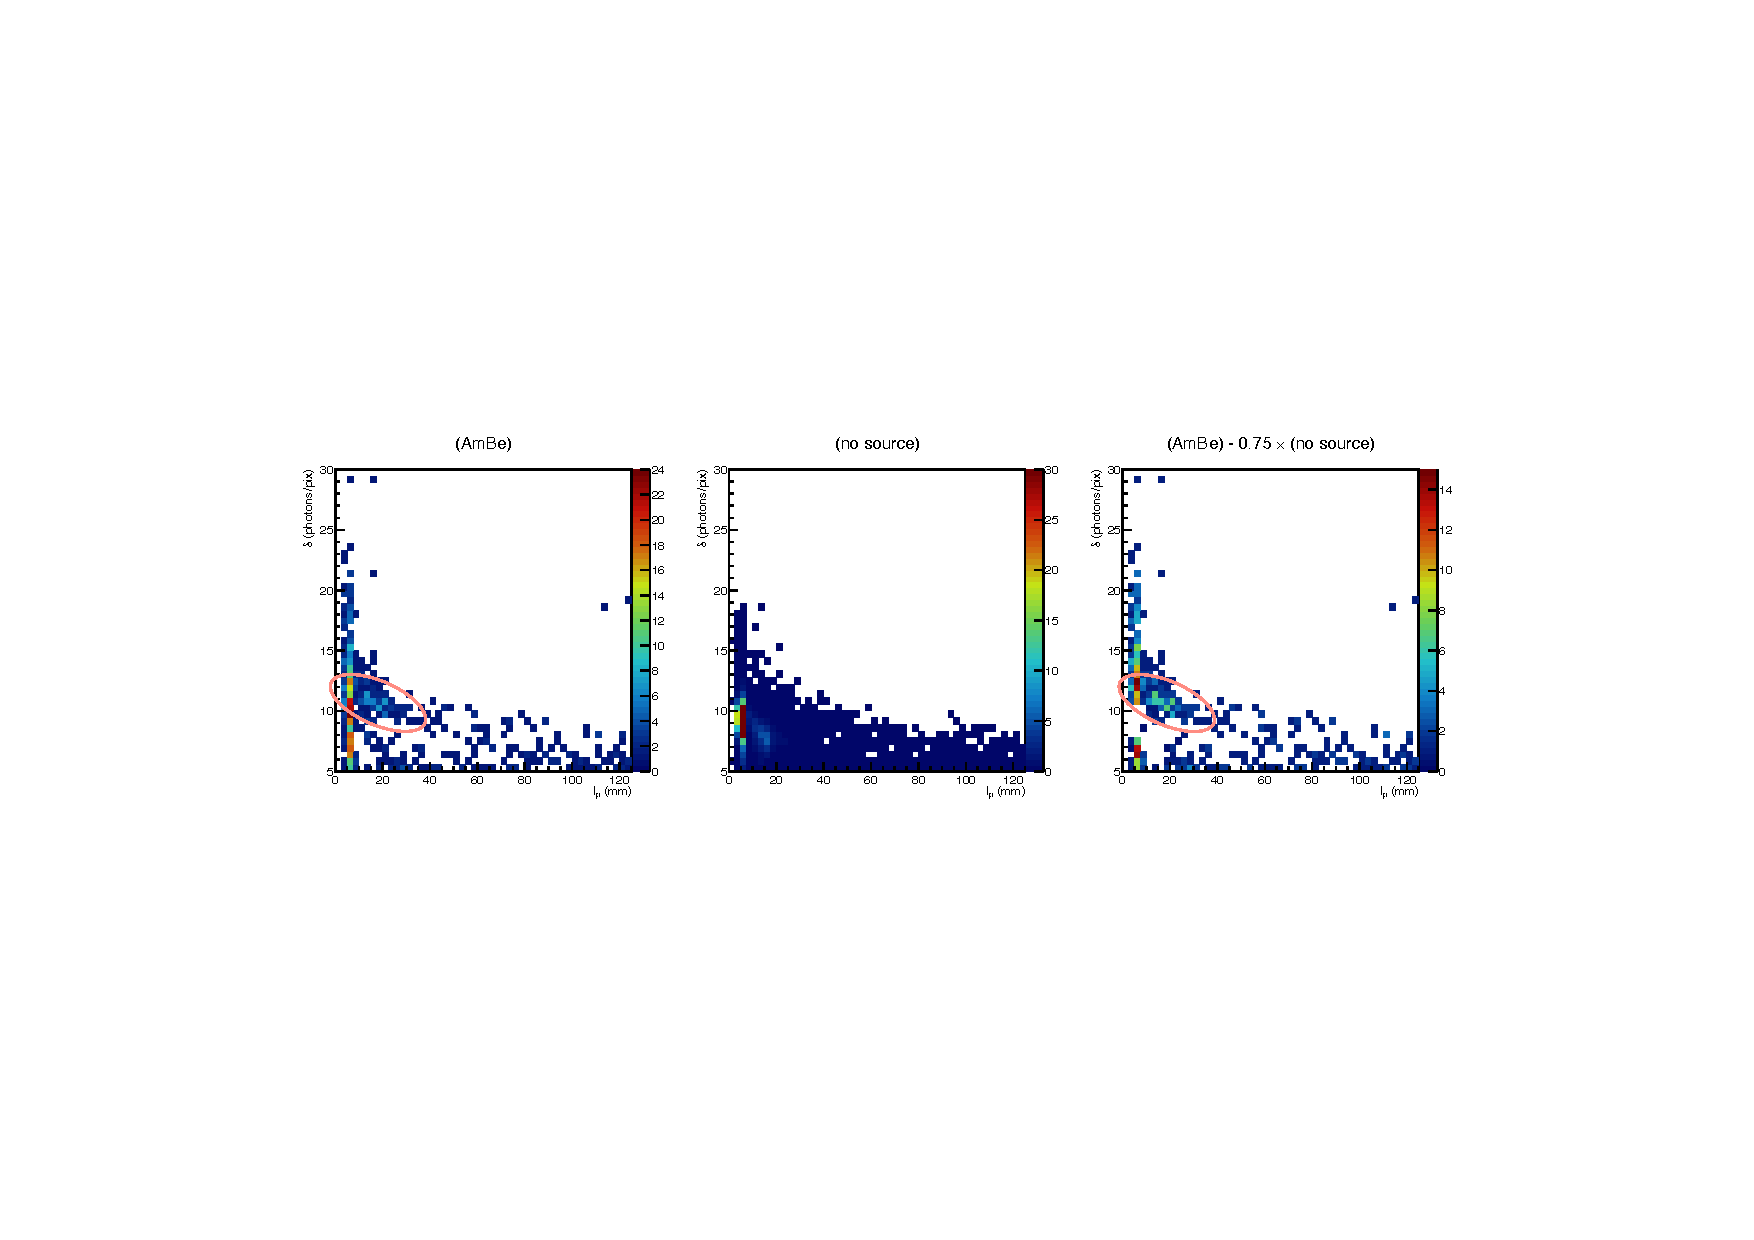
\includegraphics[width=0.90\linewidth]{figures/densityvslength_zoom}

  \caption{Supercluster light density $\delta$ versus length $l_p$,
    for data with \ambe source (left), data without any source
    (middle), and the resulting background-subtracted \ambe data.  The
    normalization of data without source is to the same exposure time
    of the \ambe one, accounting for the trigger scale factor
    $\varepsilon_{SF}$, as defined in the text. \label{fig:dvsl}}

  \end{center}
\end{figure}

\begin{figure}[ht]
  \begin{center}
  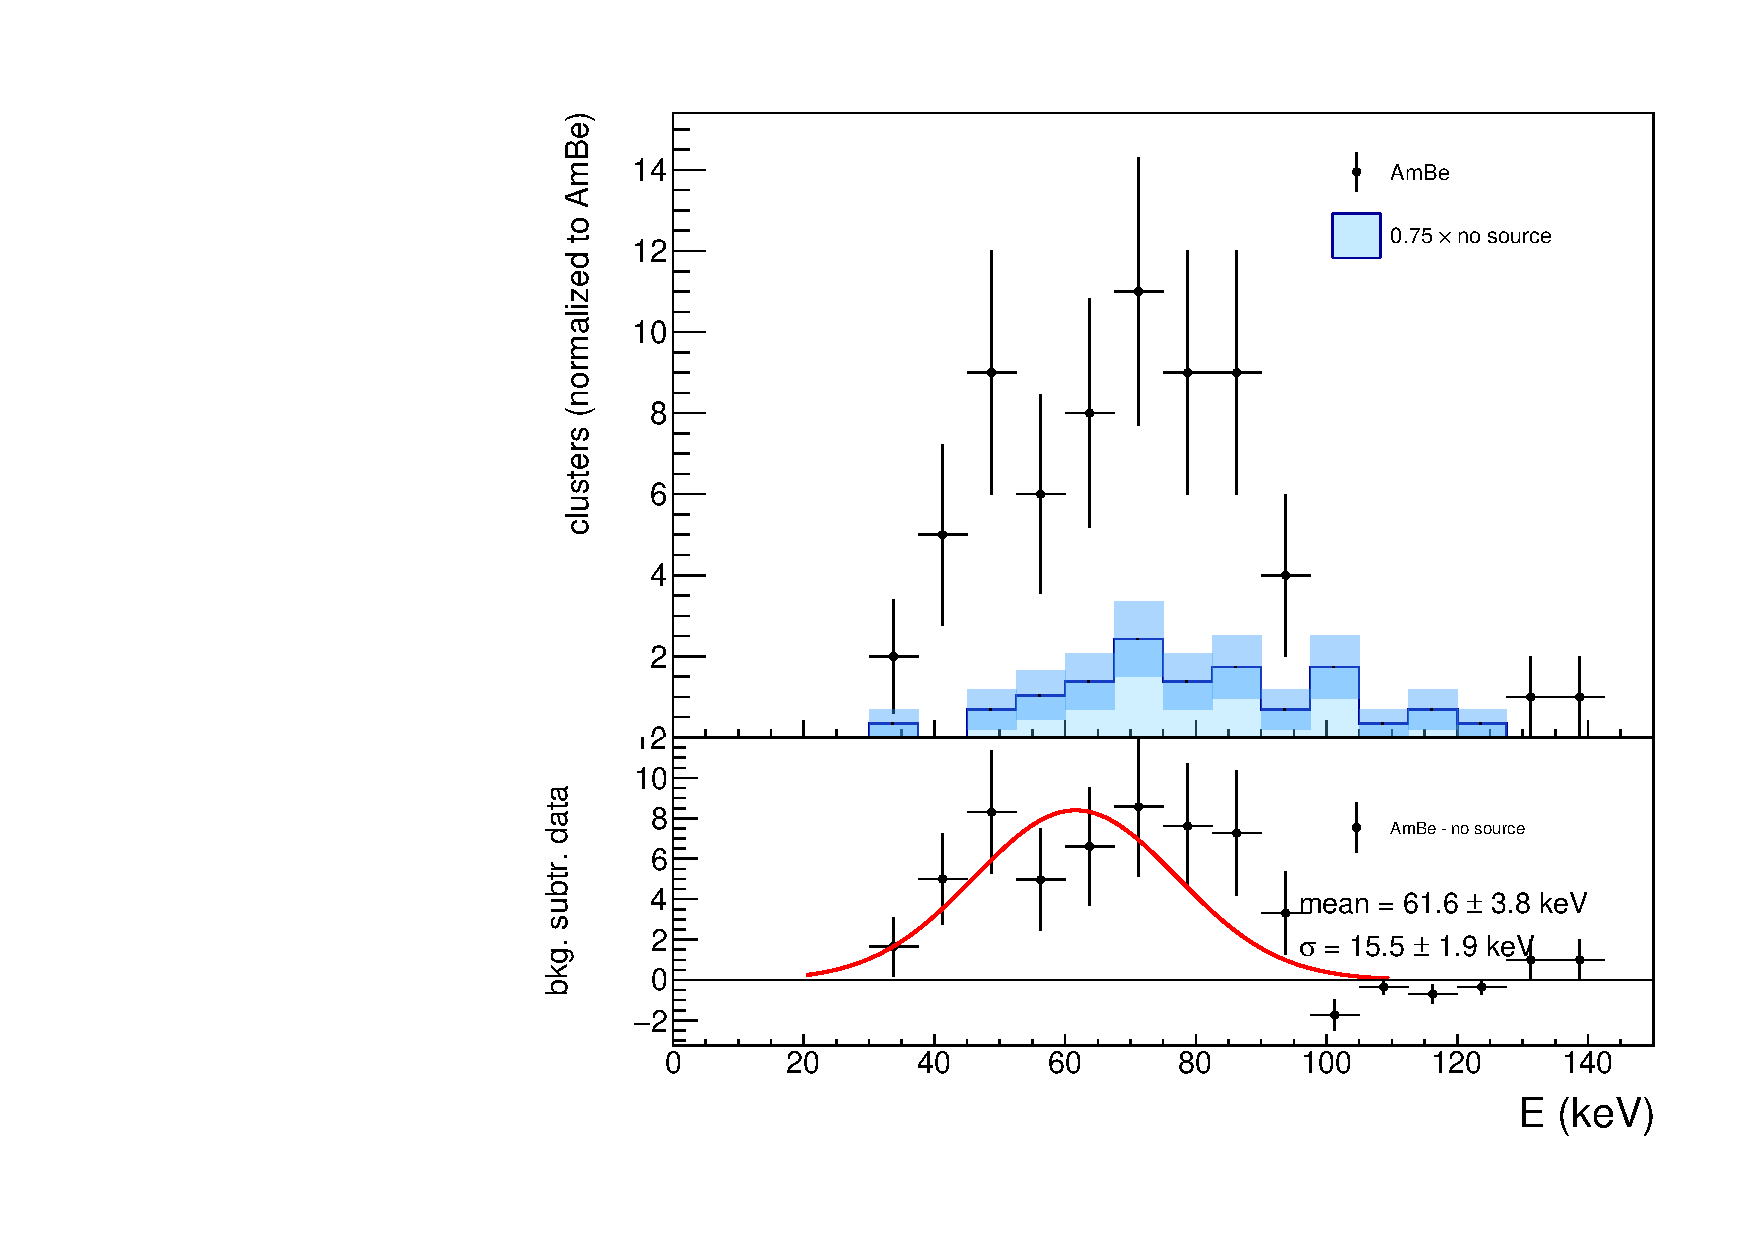
\includegraphics[width=0.60\linewidth]{figures/calintegral_59keV}

  \caption{Calibrated energy spectrum for candidates in the control
    region $PR$, as defined in the text. The background-subtracted
    distribution is fitted with a Gaussian PDF, which shows a mean
    value compatible with $E=59\keV$ expected from the $^{241}$Am
    $\gamma$s interacting with the gas. \label{fig:59keV}}

  \end{center}
\end{figure}



